% Use this template for summarizing a process building models of gene expression
\documentclass{article}
\usepackage[$margin=1in]{geometry}
\usepackage{graphicx}
\usepackage{url}
\begin{document}

\title{PCNA Role in Cell Cycle and Imaging}
\date{Wednesday, September 18, 2024}
\author{BRAD}

\maketitle

\section*{Summary of Process}
GO\_Biological\_Process\_2021

\section*{Summary of Steps}
Based on the provided text database, the role of PCNA (Proliferating Cell Nuclear Antigen) in the cell cycle and cell cycle imaging is highlighted in the context of marking the boundaries of the S phase. PCNA is mentioned as a processivity factor for DNA polymerase epsilon and delta, indicating its involvement in DNA replication during the S phase. Additionally, PCNA is used as a marker to annotate the beginning and end of the S phase in living cells, suggesting its importance in accurately delineating cell cycle phase transitions. The text also mentions that the PCNA reporter precisely marks the boundaries of the S phase, emphasizing its role in cell cycle imaging.

In summary, PCNA plays a crucial role in DNA replication during the S phase of the cell cycle and is utilized as a marker for accurately delineating cell cycle phase transitions in living cells during cell cycle imaging.\textbf{Summary:} The code was successfully executed to find the first order interactions of the gene PCNA in the Hardwired Genome. The output indicates that the script is currently in the process of finding these interactions. The next step would be to wait for the script to complete its execution and generate the output file `S<Step \texttt{number>-HWG-1stOrder-PCNA.csv}`.The 'Genes' column from the output file generated in step 2 was loaded and searched in Enrichr. The gene list was queried against the GO\_Biological\_Process\_2021 database, resulting in a table with 649 entries.

\begin{figure}
    \centering
    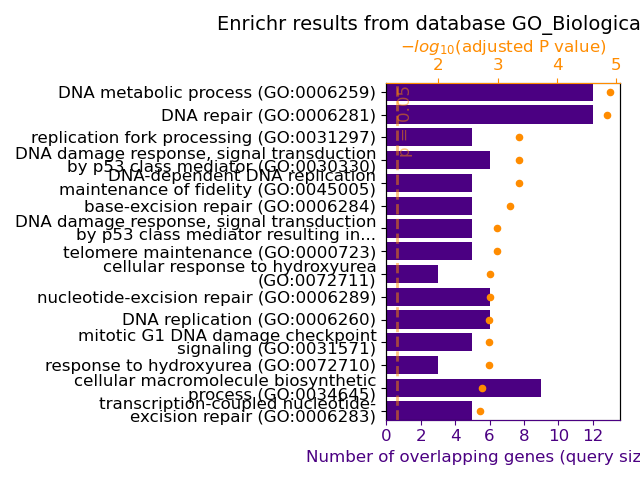
\includegraphics[width=\textwidth]{/home/jpic/RAG-DEV/tutorials/planner/output-directory/2024-09-18_11-52-21/images/S4-ENRICHR-GO_Biological_Process_2021.png}
\end{figure}



\begin{table}[h]
\centering
\begin{tabular}{rlrrrlr}
\hline
   rank & path\_name                              &       p\_val &   z\_score &   combined\_score & overlapping\_genes                                                                    &   adj\_p\_val \\
\hline
      1 & DNA-dependent DNA replication (GO:0... & 2.72468e-07 &  14.2142  &         214.858  & ['POLD3', 'MGME1', 'POLA1', 'WRN', 'PSMB5', 'REV3L', 'HMGA1', 'PSMA7']               & 0.000192635 \\
      2 & mRNA 3'-end processing (GO:0031124)... & 2.7791e-06  &  17.3363  &         221.79   & ['DDX39A', 'CPSF3', 'CSTF1', 'RNPS1', 'PAPOLB', 'MAGOHB']                            & 0.000982413 \\
      3 & RNA splicing, via transesterificati... & 4.71279e-06 &   8.03388 &          98.5373 & ['DDX39A', 'NONO', 'CPSF3', 'CSTF1', 'POLR2F', 'RNPS1', 'SNRPB2', 'SNRPC', 'MAGOHB'] & 0.00111065  \\
      4 & mRNA splicing, via spliceosome (GO:... & 9.55686e-06 &   7.32801 &          84.699  & ['DDX39A', 'NONO', 'CPSF3', 'CSTF1', 'POLR2F', 'RNPS1', 'SNRPB2', 'SNRPC', 'MAGOHB'] & 0.0015436   \\
      5 & mitotic spindle organization (GO:00... & 1.39542e-05 &   9.91039 &         110.796  & ['INTS13', 'INCENP', 'CHEK2', 'MIS12', 'CENPM', 'RANGAP1', 'SMC1A']                  & 0.0015436   \\
      6 & tRNA modification (GO:0006400)...      & 1.83979e-05 &  17.4035  &         189.755  & ['MOCS3', 'WDR4', 'FTSJ1', 'OSGEP', 'ADAT2']                                         & 0.0015436   \\
      7 & double-strand break repair (GO:0006... & 1.85146e-05 &   9.46517 &         103.142  & ['POLA1', 'XRCC6', 'WRN', 'POLN', 'CHEK2', 'REV3L', 'SMC6']                          & 0.0015436   \\
      8 & DNA repair (GO:0006281)...             & 1.86389e-05 &   6.71124 &          73.0872 & ['POLD3', 'MGME1', 'POLA1', 'WRN', 'POLN', 'CHEK2', 'SMC1A', 'RAD23B', 'MLH3']       & 0.0015436   \\
      9 & mRNA processing (GO:0006397)...        & 1.96497e-05 &   6.66444 &          72.2255 & ['DDX39A', 'NONO', 'CPSF3', 'CSTF1', 'POLR2F', 'RNPS1', 'SNRPB2', 'SNRPC', 'MAGOHB'] & 0.0015436   \\
     10 & RNA 3'-end processing (GO:0031123)...  & 2.46401e-05 &  16.3125  &         173.094  & ['DDX39A', 'CPSF3', 'CSTF1', 'RNPS1', 'MAGOHB']                                      & 0.00174206  \\
     11 & tRNA wobble base modification (GO:0... & 4.24153e-05 &  55.9203  &         563.006  & ['MOCS3', 'ELP3', 'ADAT2']                                                           & 0.00272615  \\
     12 & DNA synthesis involved in DNA repai... & 6.25094e-05 &  21.219   &         205.404  & ['POLD3', 'POLA1', 'WRN', 'POLN']                                                    & 0.00368285  \\
     13 & DNA biosynthetic process (GO:007189... & 7.83783e-05 &  43.9308  &         415.32   & ['POLD3', 'POLA1', 'WRN']                                                            & 0.00426257  \\
     14 & telomere maintenance (GO:0000723)...   & 0.000177012 &  15.9038  &         137.398  & ['POLD3', 'WRN', 'XRCC6', 'SMC6']                                                    & 0.0089391   \\
     15 & regulation of mitotic cell cycle (G... & 0.000272588 &   7.32113 &          60.0885 & ['INTS13', 'BORA', 'PSMB5', 'CKS2', 'UBE2D1', 'PSMA7']                               & 0.012848    \\
     16 & microtubule cytoskeleton organizati... & 0.000459779 &   8.46256 &          65.0328 & ['INTS13', 'INCENP', 'MIS12', 'CENPM', 'RANGAP1']                                    & 0.0203165   \\
     17 & recombinational repair (GO:0000725)... & 0.000663247 &  11.0139  &          80.6036 & ['WRN', 'POLN', 'REV3L', 'SMC6']                                                     & 0.0266914   \\
     18 & isoprenoid metabolic process (GO:00... & 0.000679555 &  67.6667  &         493.566  & ['PDSS2', 'PDSS1']                                                                   & 0.0266914   \\
     19 & isoprenoid biosynthetic process (GO... & 0.000870867 &  57.9971  &         408.649  & ['PDSS2', 'PDSS1']                                                                   & 0.0324054   \\
     20 & translesion synthesis (GO:0019985)...  & 0.00120859  &  15.7502  &         105.815  & ['POLD3', 'POLN', 'REV3L']                                                           & 0.0427237   \\
\hline
\end{tabular}
\end{table}


% \subsection{Data}
% {BRAD PUT SUMMARY OF DATASET}

% \subsection{Coordinates}
% {BRAD DISCUSS THE DATA REPRESENTATION}

% \subsection{Model}
% {BRAD DISCUSS THE MODEL}

% \subsection{Analysis}
% {BRAD DISCUSS THE ANALYSIS}



\end{document}
